Energy price prediction is a cumbersome task to handle because of the highly volatile nature of price prediction and the plethora of factors that influence the energy price. In this section we will show the factors that influence the price by analysing relevant data that will later become input in our ANN. Not to surprisingly; the most important factor in any market is demand and this greatly influences the price "REFERENCE". But also time of day, day of the week, wind speed and temperature (which are the quantifiable factors) play a big role. Sociocultural influences affects the price as well but are hard to measure. This section will show the connection between energy price and some of the influential factors.
\todo{Make reference to earlier work in the thesis}
\todo{Lav reference til tidligere omkring seasonality og de ting der spiller ind.}
\todo{Uddyb introen til afsnittet.}

%Table ~\ref{table:pearsonCoeficientPrice} shows the correlation coefficient between factors that have been discussed earlier as having an influence on the electricity price. As discussed in the wind production section the correlation coefficient is a value between -1 and +1 that represents the linear dependency between two variables. 

%\begin{table}[H]
%\centering  % used for centering table
%\begin{tabular}{c c} % centered columns (3 columns)
%Input factor \#1 & Pearson Correlation Coefficient \\ [0.5ex] % inserts table 
%heading
%\hline                  % inserts single horizontal line
%Consumption & 0.281301381724 \\ % inserting body of the table
%Wind Speed & -0.271821873508 \\
%Temperature & -0.147262088023 \\
%Wind Direction & -0.161895363332 \\ [1ex] % [1ex] adds vertical space
%\hline %inserts single line
%\end{tabular}
%\caption{Table showing Pearson correlation coefficient between various factors and the price.} % title of Table
%\label{table:pearsonCoeficientPrice} % is used to refer this table in the text
%\end{table}

\subsection{Price}\label{sec:Price}
We present some of the influences on the price in this section and argue why these parameters have an impact on the price. We also account for the time perspective of the price and show the non-linear nature of energy prices. Since we just talked about demand and the influence on price we are focusing on the other impacting factors in the prediction of energy prices \todo{demand is not above?}. To accompany the graphs we also calculated the Pearson's correlations (section ~\ref{sec:Pearsons}) which can be seen in table ~\ref{table:pearsonsPriceVariables}.

Pearson's correlations:
\begin{table}[H]
\centering  % used for centering table
\begin{tabular}{c c} % centered columns
 \#0 Parameters & \#1 Pearsons \\ [0.5ex] % inserts table 
%heading
\hline                  % inserts single horizontal line
Price/Demand & 0.310686748459 \\
Price/Wind speed & -0.278480552449  \\
Price/Temperature & -0.175026569339 \\
Demand/Wind speed & 0.567853517055 \\
Demand/Temperature & -0.592827186022 \\
\hline %inserts single line
\end{tabular}
\caption{Pearson's correlations for price prediction variables} % title of Table
\label{table:pearsonsPriceVariables} % is used to refer this table in the text
\end{table}

\subsubsection{Weather conditional influences}
The electricity price is affected by different weather conditions. We present temperature and wind speed and show how they influence the price.

\begin{figure}[H]
\centering
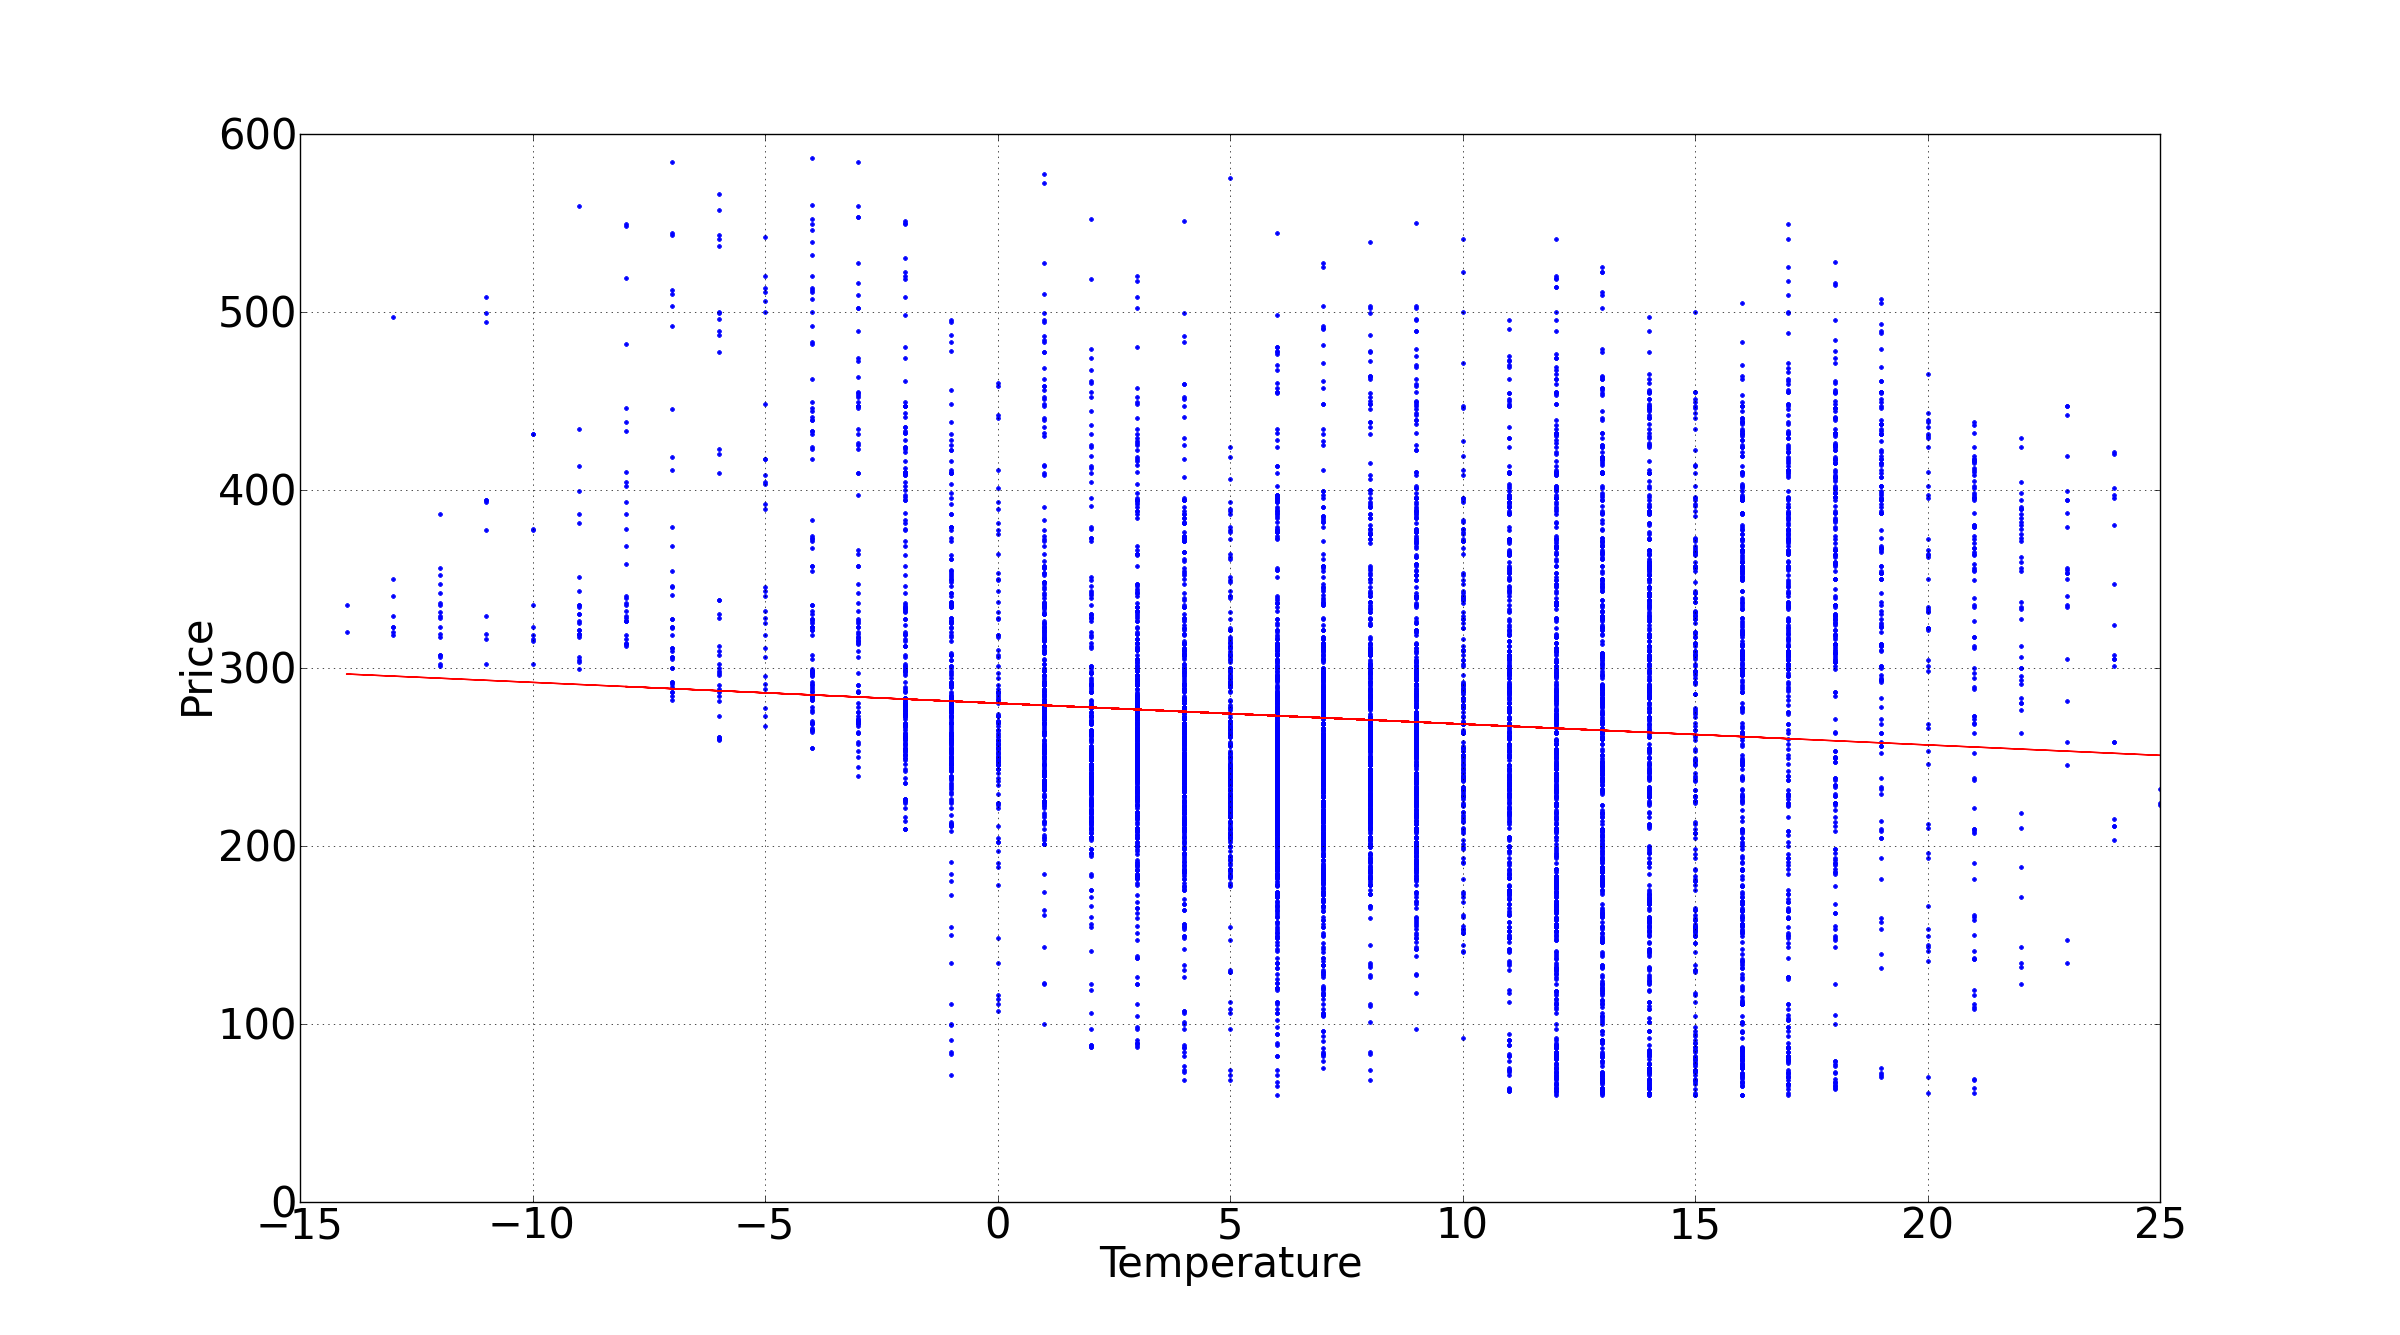
\includegraphics[width=0.8\textwidth ]{billeder/energy_price_plots/price_temp.png}
\caption{Price and temperature plot.}
\label{fig:price_temp}
\end{figure}

In figure~\ref{fig:price_temp} and table~\ref{table:pearsonsPriceVariables} we see that there is nearly no correlation between temperature and the price. This indicates that we cannot use the temperature as a direct input to the ANN. But the temperature has an indirect influence on the price since it has an influence on the demand. This variable is only used to substitute the demand to make our prediction self-contained. This will be discussed later.

\begin{figure}[H]
\centering
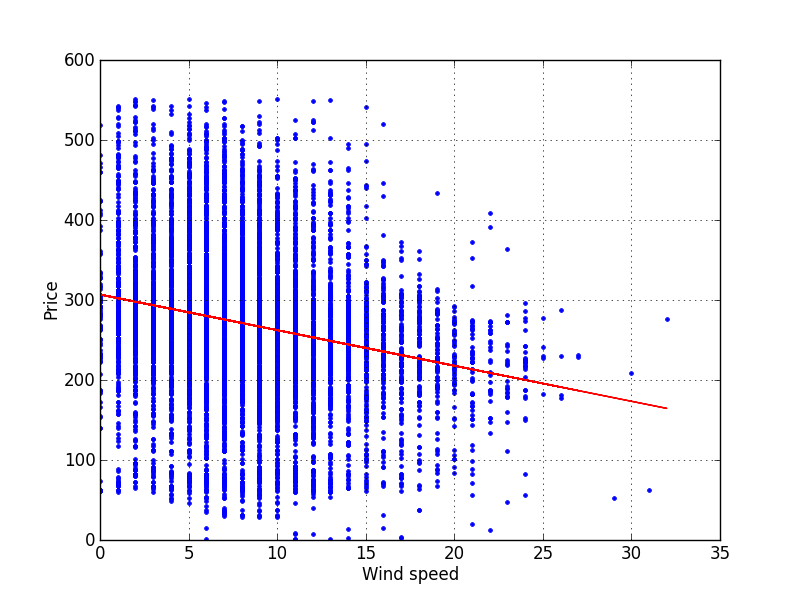
\includegraphics[width=0.8\textwidth ]{billeder/energy_price_plots/price_wind.png}
\caption{Price and wind speed plot.}
\label{fig:price_wind}
\end{figure}

In Figure ~\ref{fig:price_wind} we see how the wind impacts the price. If the wind speed increases the energy price decreases this agrees with paper \cite{dayAheadImpactOfWindPowerForecasts} where they show that the wind influences the wind power production. The share of green energy produced from wind mills are approximately 25\% as off 2008(\cite{windPowerDanishLiberalized}) so we expect to see the wind has an impact on the price. When the production is high and the demand is moderate the price will decrease because of overproduction and since we cannot store energy for later use the price will drop.
\todo{Snak om distributionen. Det skal ikke ses som en 1-til-1, men som en variabel der kan sende prisen i den rigtige retning.}

\subsection{Seasonality}\label{sec:seasonality}
The price is influenced greatly by the seasonality. Seasonality covers the time of year but also the time-of-day and the day-of-the-week in this section. Sesonality plays a significant role in price prediction because the demand is affected by the consumption of the people and since people follow patterns the demand does aswell.
\todo{Make section about seasonality in general}
\begin{figure}[H]
\centering
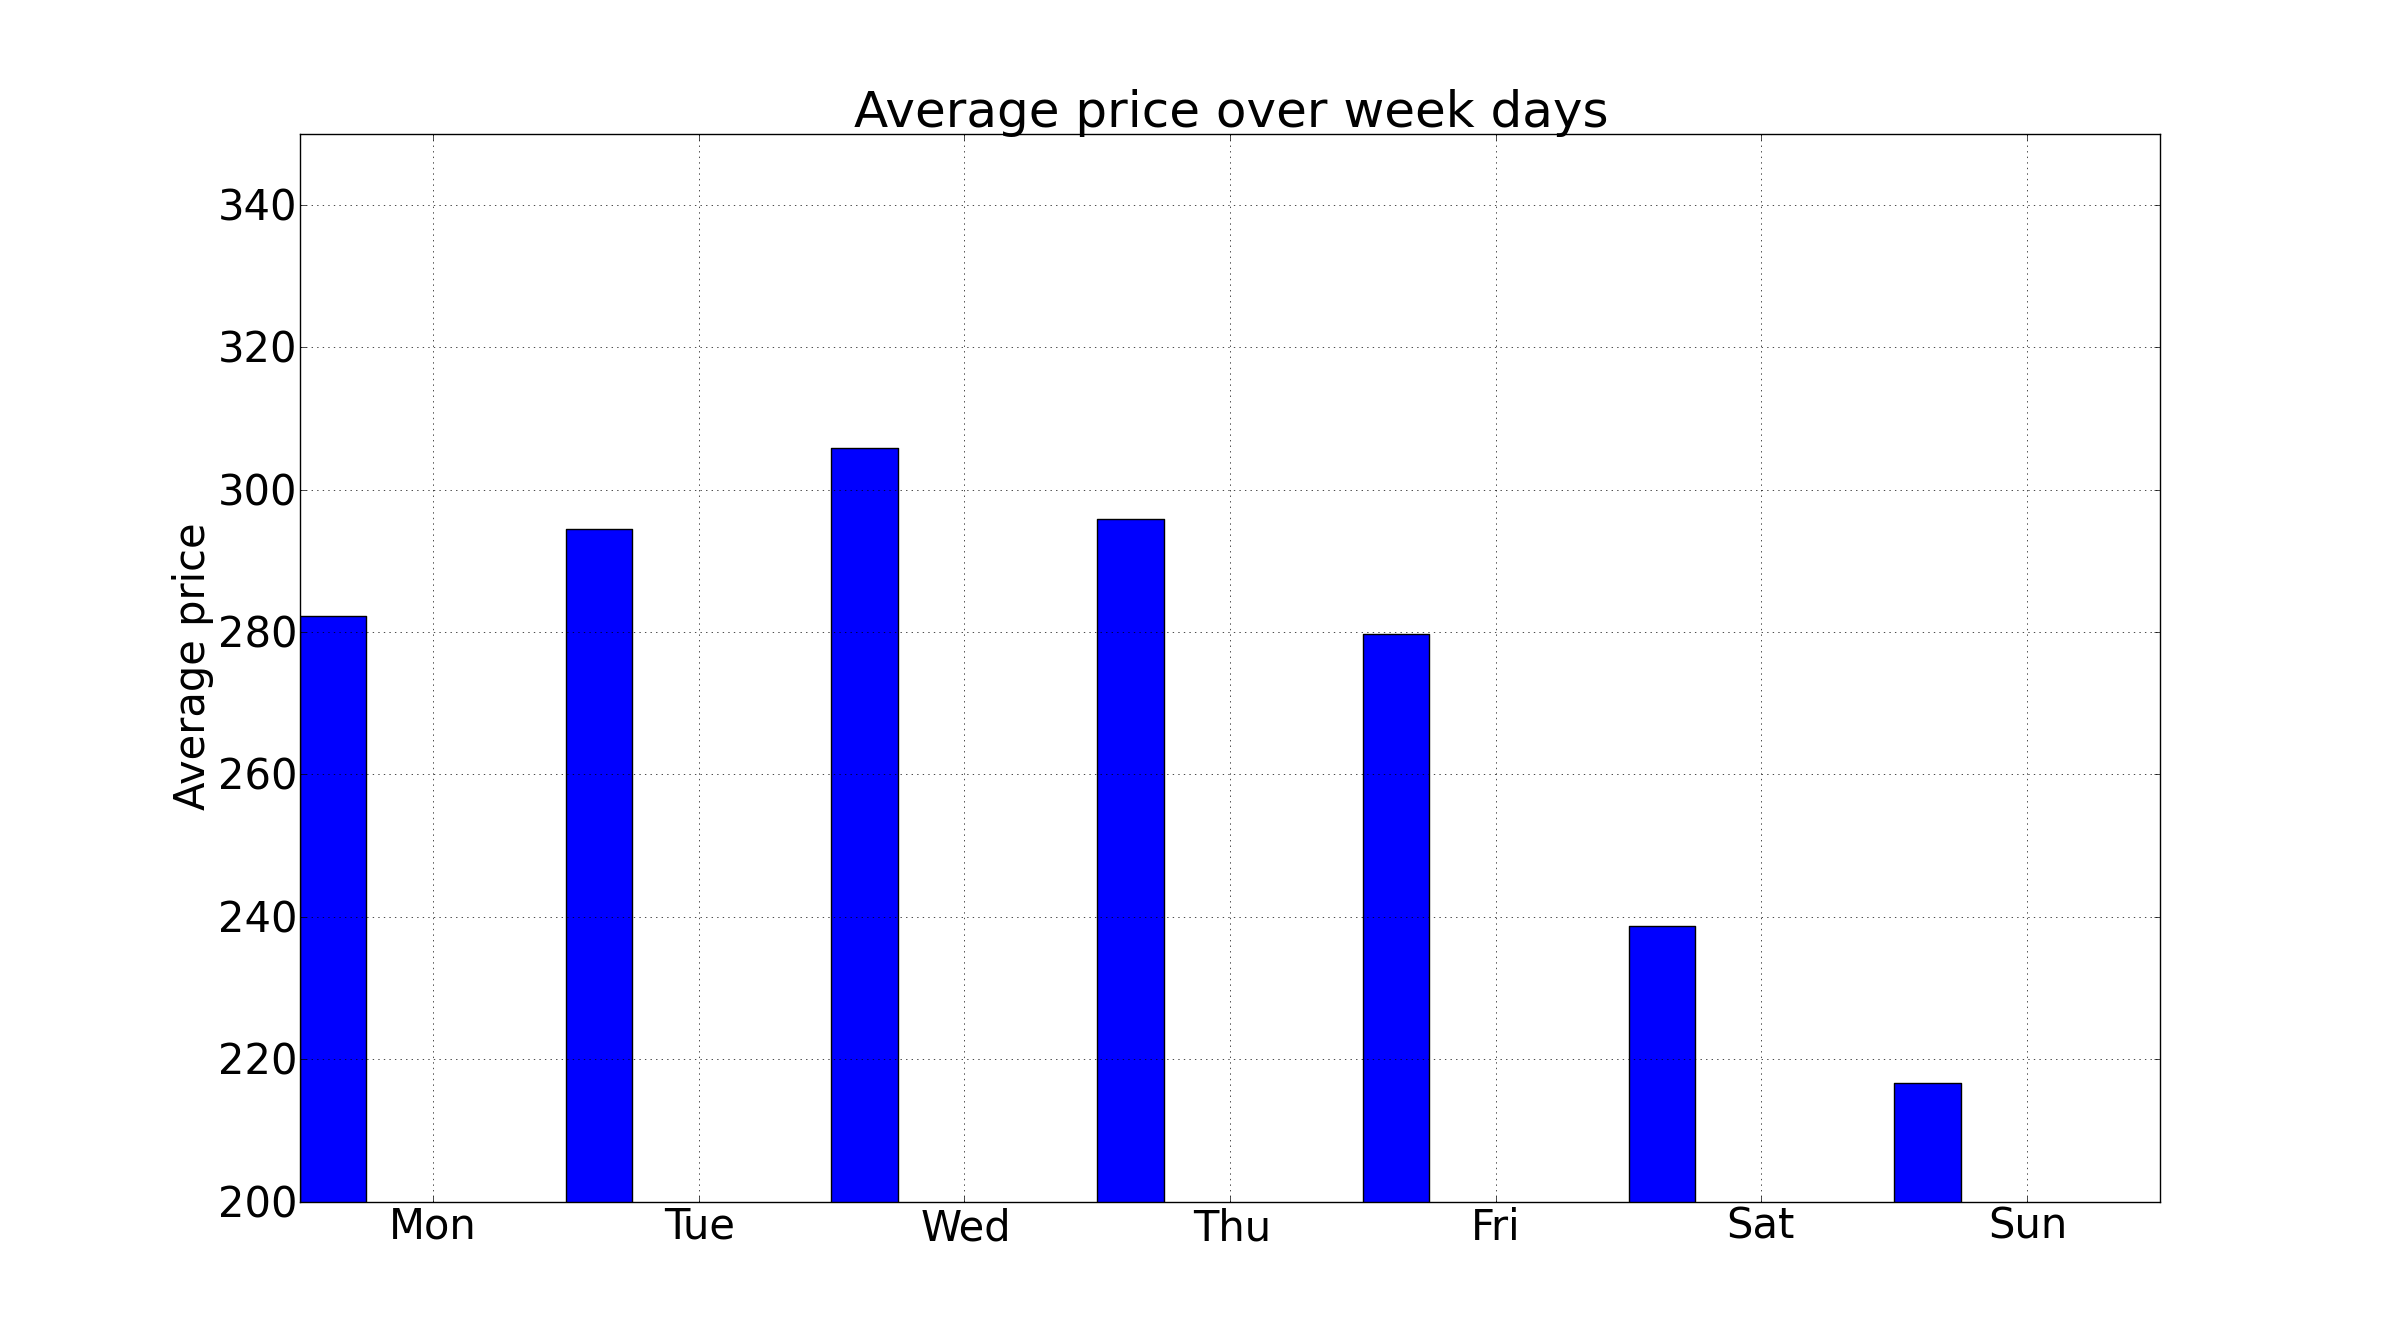
\includegraphics[width=0.8\textwidth ]{billeder/energy_price_plots/Average_price_over_weekdays.png}
\caption{Daily price dispersion}
\label{fig:price_over_weekdays}
\end{figure}

Figure ~\ref{fig:price_over_weekdays} shows us how the trend of the price varies over the different days in a week. The most noticeable here is how the price is decreasing in the weekend (Saturday and Sunday) and are somewhat steady for the weekdays. We are looking at two options for our neural network. We can represent it as a matrix (section ~\ref{sec:Matrix}) which is the most granulated method. We can also normalize the days 1-7 and represent all days with only 1 input neuron.
The graph show us a difference between highest (Wednesday) and lowest (Sunday) of 80 which is pretty much when the price fluctuates between 632 and 61 (with 1\% top and bottom trim see section ~\ref{sec:Trimming}).

\begin{figure}[H]
\centering
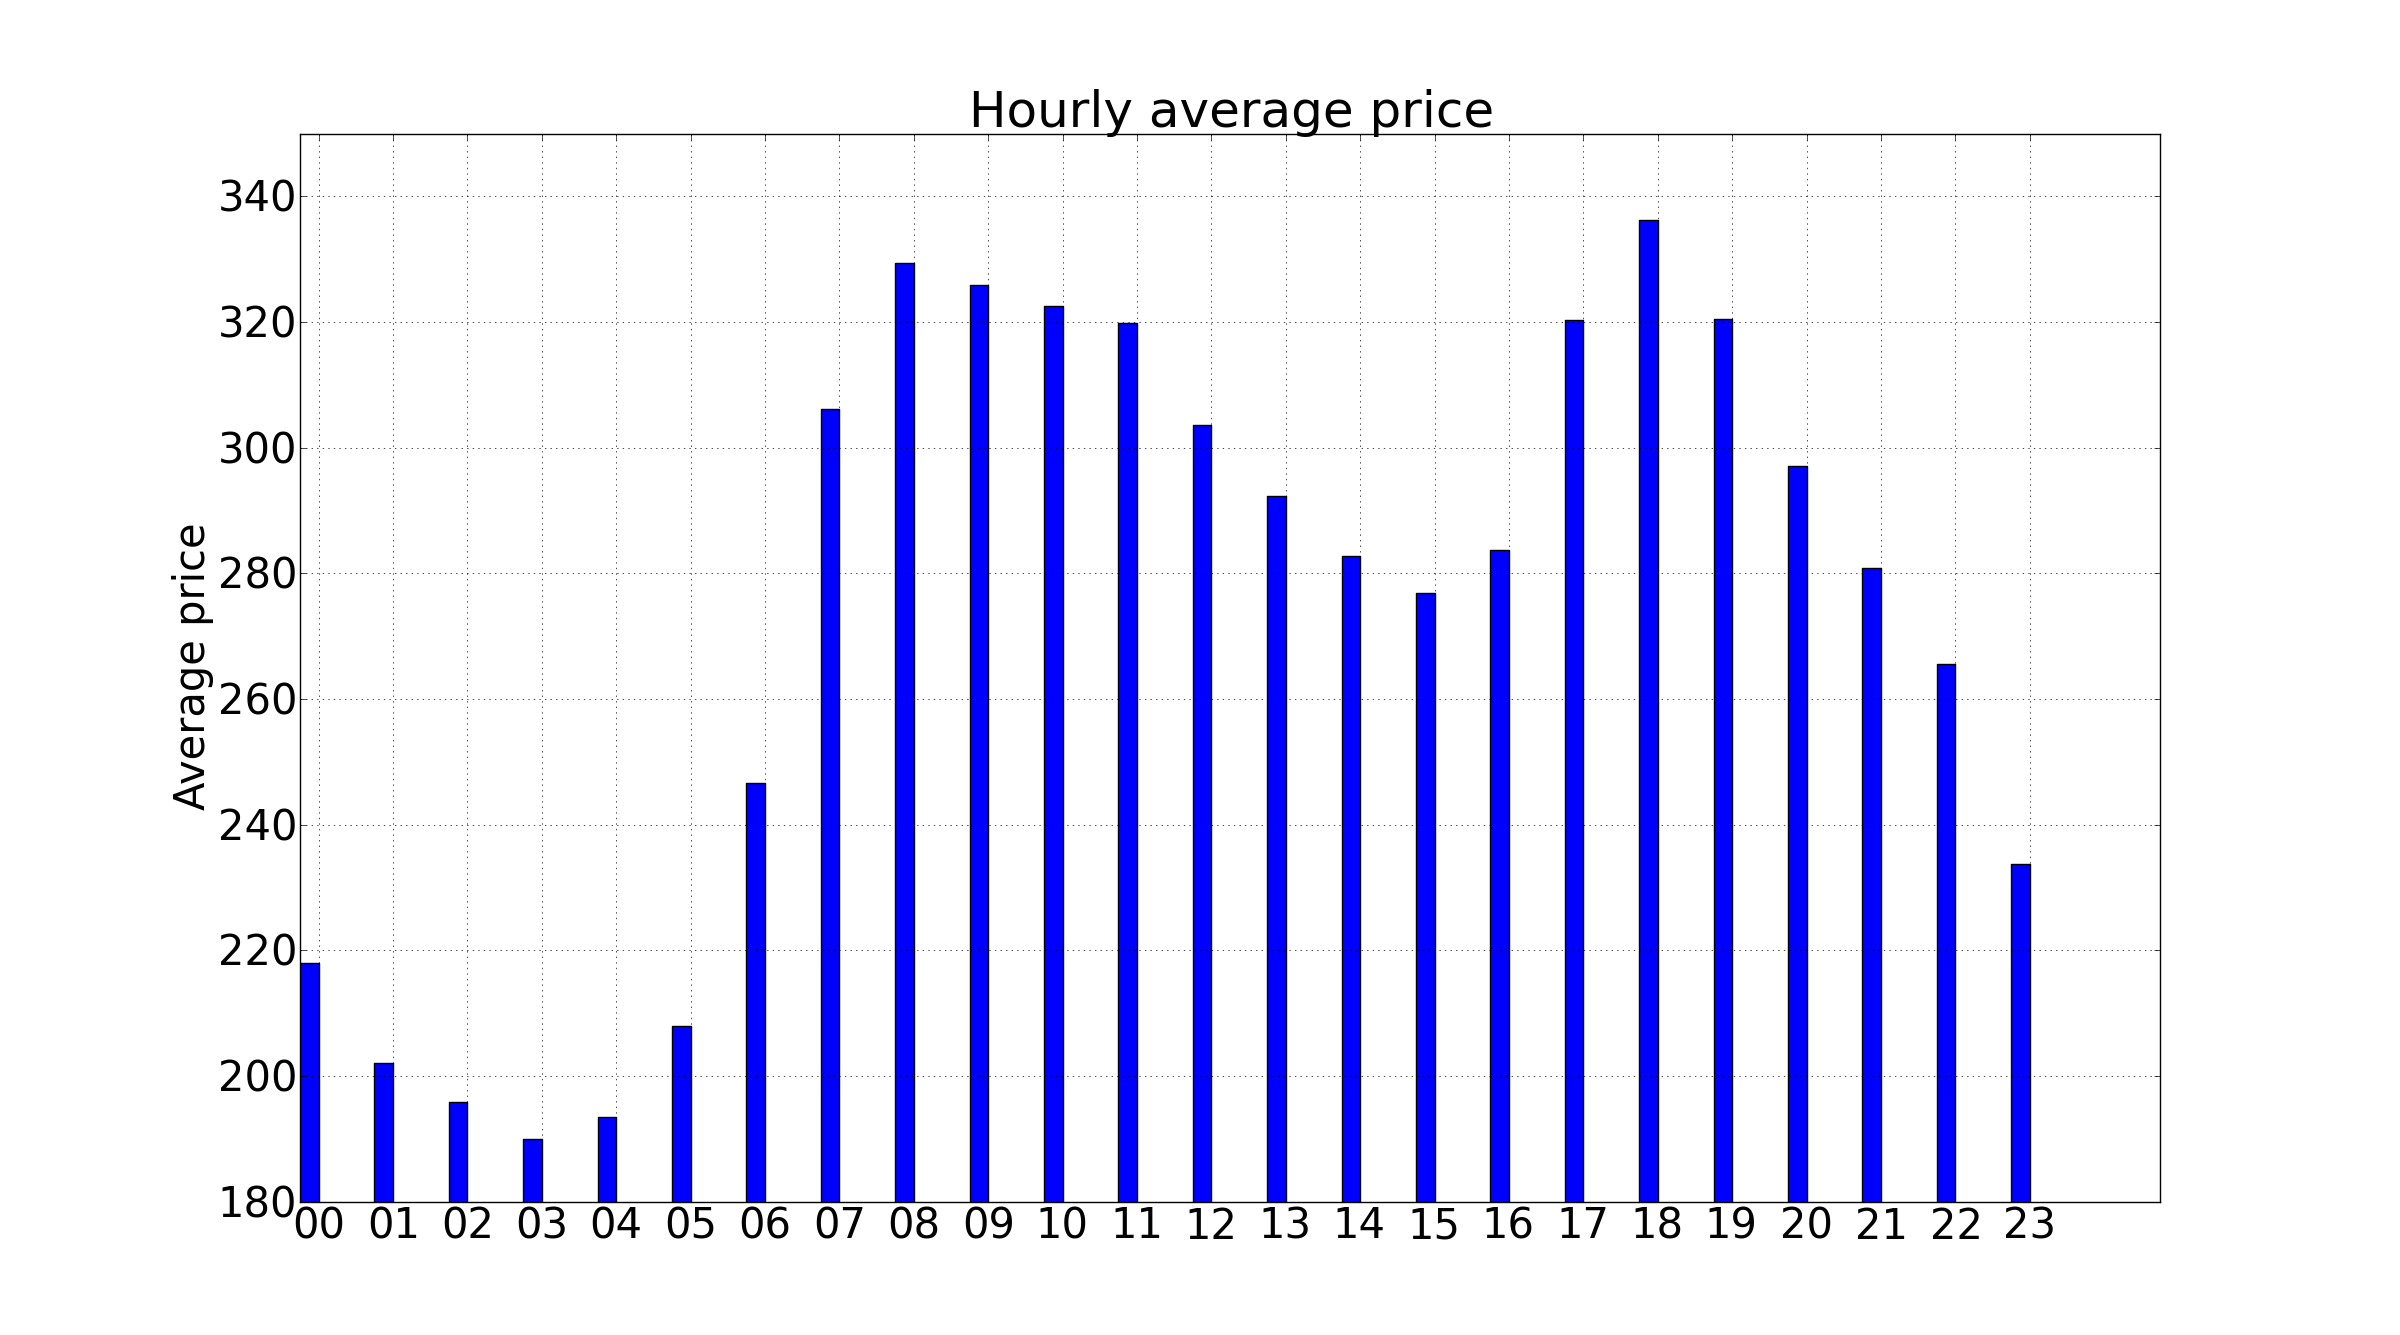
\includegraphics[width=0.8\textwidth ]{billeder/energy_price_plots/price_per_hour.png}
\caption{Hourly price dispersion}
\label{fig:price_per_hour}
\end{figure}

In Figure~\ref{fig:price_per_hour} we see the average price per hour over a whole day. We see a trend where the price is highest from 08 to 10 and again from 17 to 19. This is because most people wake up in the first interval and use a lot of electricity and the second interval is when everybody gets home and cooks dinner. The price can be represented (as described in price-over-weekdays) as a matrix or a single normalized input. The price fluctuates between 335(18) and 190(03) which gives us a difference of 145. This is a pretty significant difference between highest and lowest and will help us point the prediction in the right direction.

\begin{figure}[H]
\centering
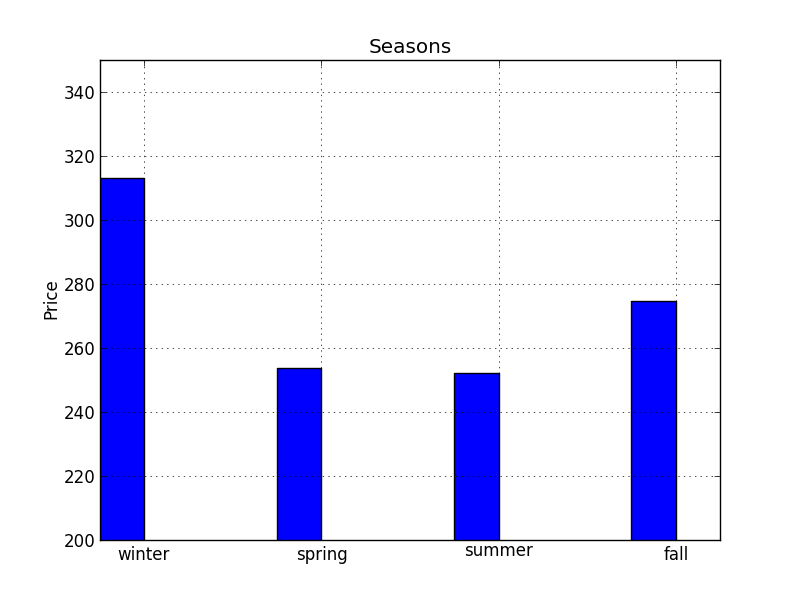
\includegraphics[width=0.8\textwidth ]{billeder/energy_price_plots/seasons.png}
\caption{Seasonal price dispersion}
\label{fig:seasons}
\end{figure}

The sesonality is also reflected in what time of year it is. In the winter time the electrical heating and need for electric light plays a significant role on how much electricity is consumed and thus the price goes up. This is shown in figure ~\ref{fig:seasons} where it clearly shows the average price is higher in winter and fall than in summer and spring.

\begin{figure}[H]
\centering
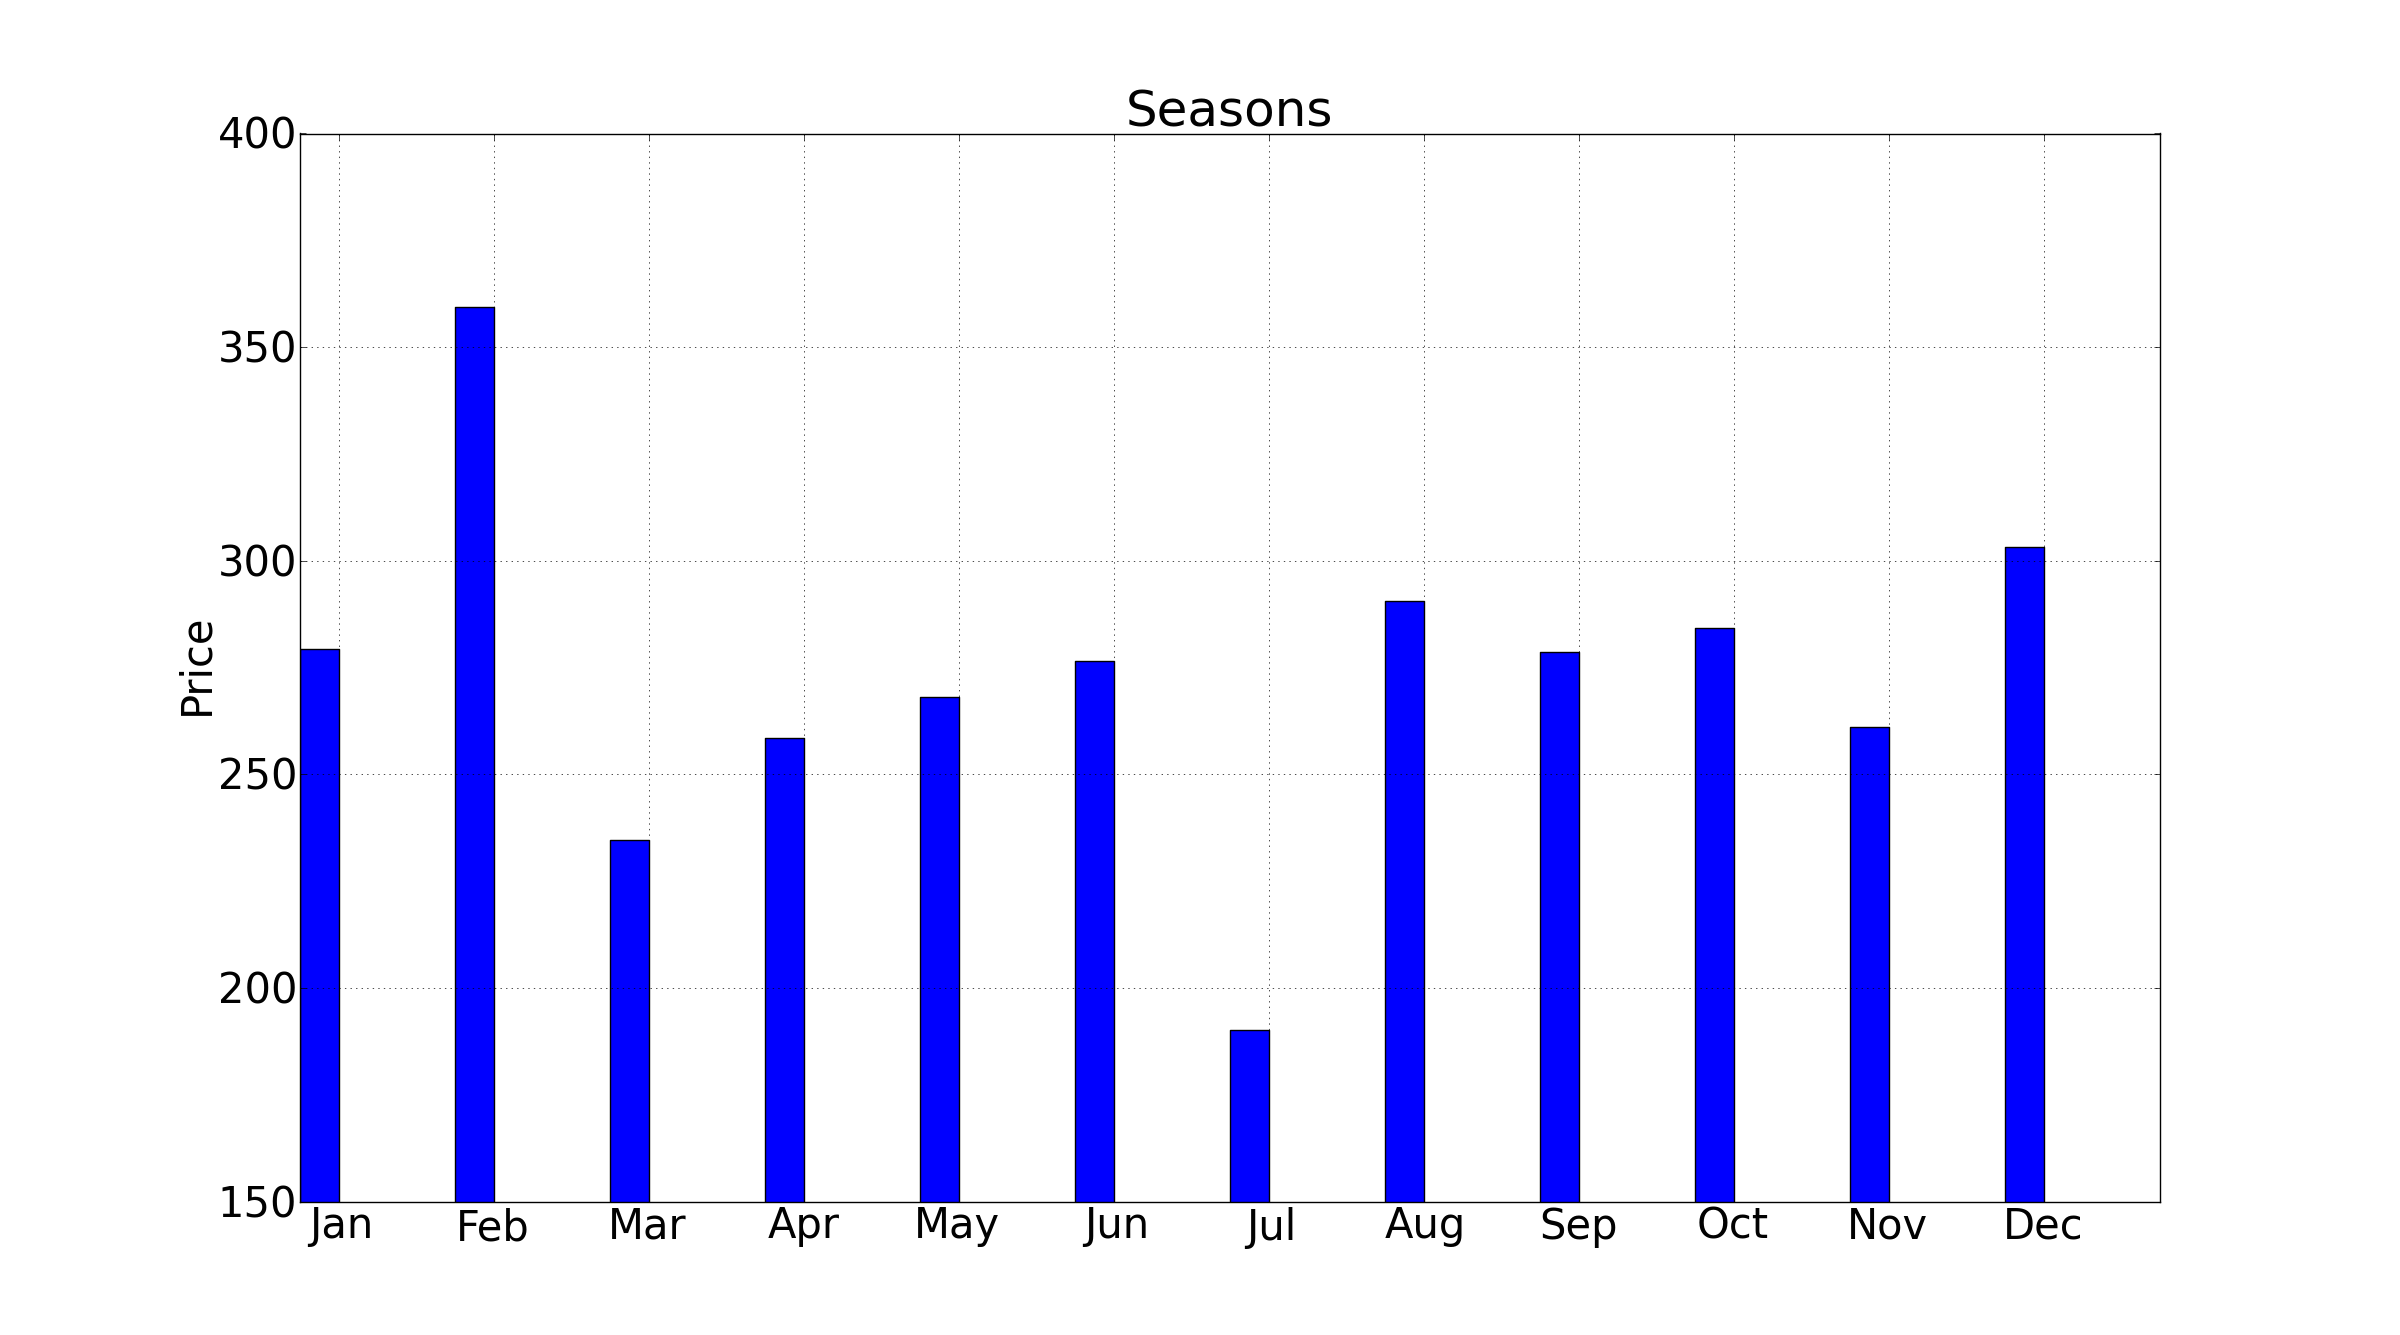
\includegraphics[width=0.8\textwidth ]{billeder/energy_price_plots/averageMonthlyPrice.png}
\caption{Monthly price dispersion}
\label{fig:monthlyAveragePrice}
\end{figure}

To get a more fine grained representation of the seasonal influences on the price; we created a monthly distribution of the price. The figure ~\ref{fig:monthlyAveragePrice} shows that the highest average price is 360(february) and lowest 190(july). This is a significant price jump and shows the same trend as for the seasonal figure ~\ref{fig:seasons} but here we see the effects of the holidays in july; where the price is significantly lower than the rest of the year.

\subsection{Volatility and High-Frequency}
The energy prices are very volatile and changes on an hourly basis. The volatility is often reflected in the same conditions for the hour gives completely different results. In addition to the volatility the price has a very high frequence of spike prices. A spike price is a price that elavates very quickly and drops in a matter of a few hours. These conditions can be tricky to handle but we will here address some of the problems in handling volatility and spike prices.

\begin{figure}[H]
\centering
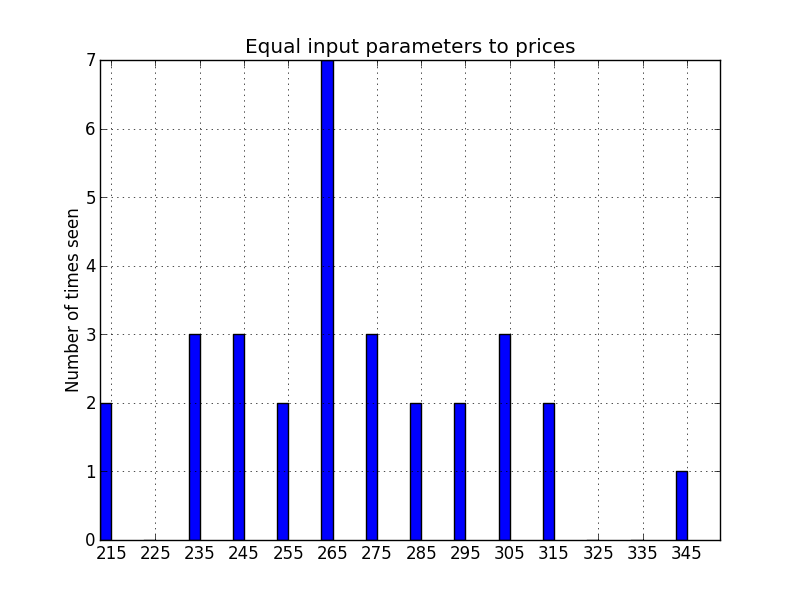
\includegraphics[width=0.8\textwidth ]{billeder/energy_price_plots/same_hour_distribution.png}
\caption{Price ditribution over equal hours}
\label{fig:same_hour_distribution}
\end{figure}

In earlier figures we have shown how the input influences the price and given some reasons to why this influences the price. In figure~\ref{fig:same_hour_distribution} we have chosen similar hours across all days of a year and we show how different the price can be for similar inputs. The similar days have been chosen from the 'core' inputs (wind speed, temperature and demand) and the margins seen in table~\ref{table:similarHoursLimits} reflects the upper and lower bound of the inputs. The margins are calculated from a randomly chosen day and the interval is 10\% up and down. Even though the price is volatile we can see a trend in the graph that shows us that the price most of the time will be about 265.

\begin{table}[H]
\centering  % used for centering table
\begin{tabular}{c c c c} % centered columns (3 columns)
 & \#1 Windspeed & \#2 Temperature & \#3 Demand \\ [0.5ex] % inserts table 
%heading
\hline                  % inserts single horizontal line
High margin: & 12.1 & 6.6 & 2510  \\
Low margin: & 9.9 & 5.4 & 2053 \\ [1ex] % [1ex] adds vertical space
\hline %inserts single line
\end{tabular}
\caption{This is the high and low margins for our similar hours comparison.} % title of Table
\label{table:similarHoursLimits} % is used to refer this table in the text
\end{table}

\begin{figure}[H]
\centering
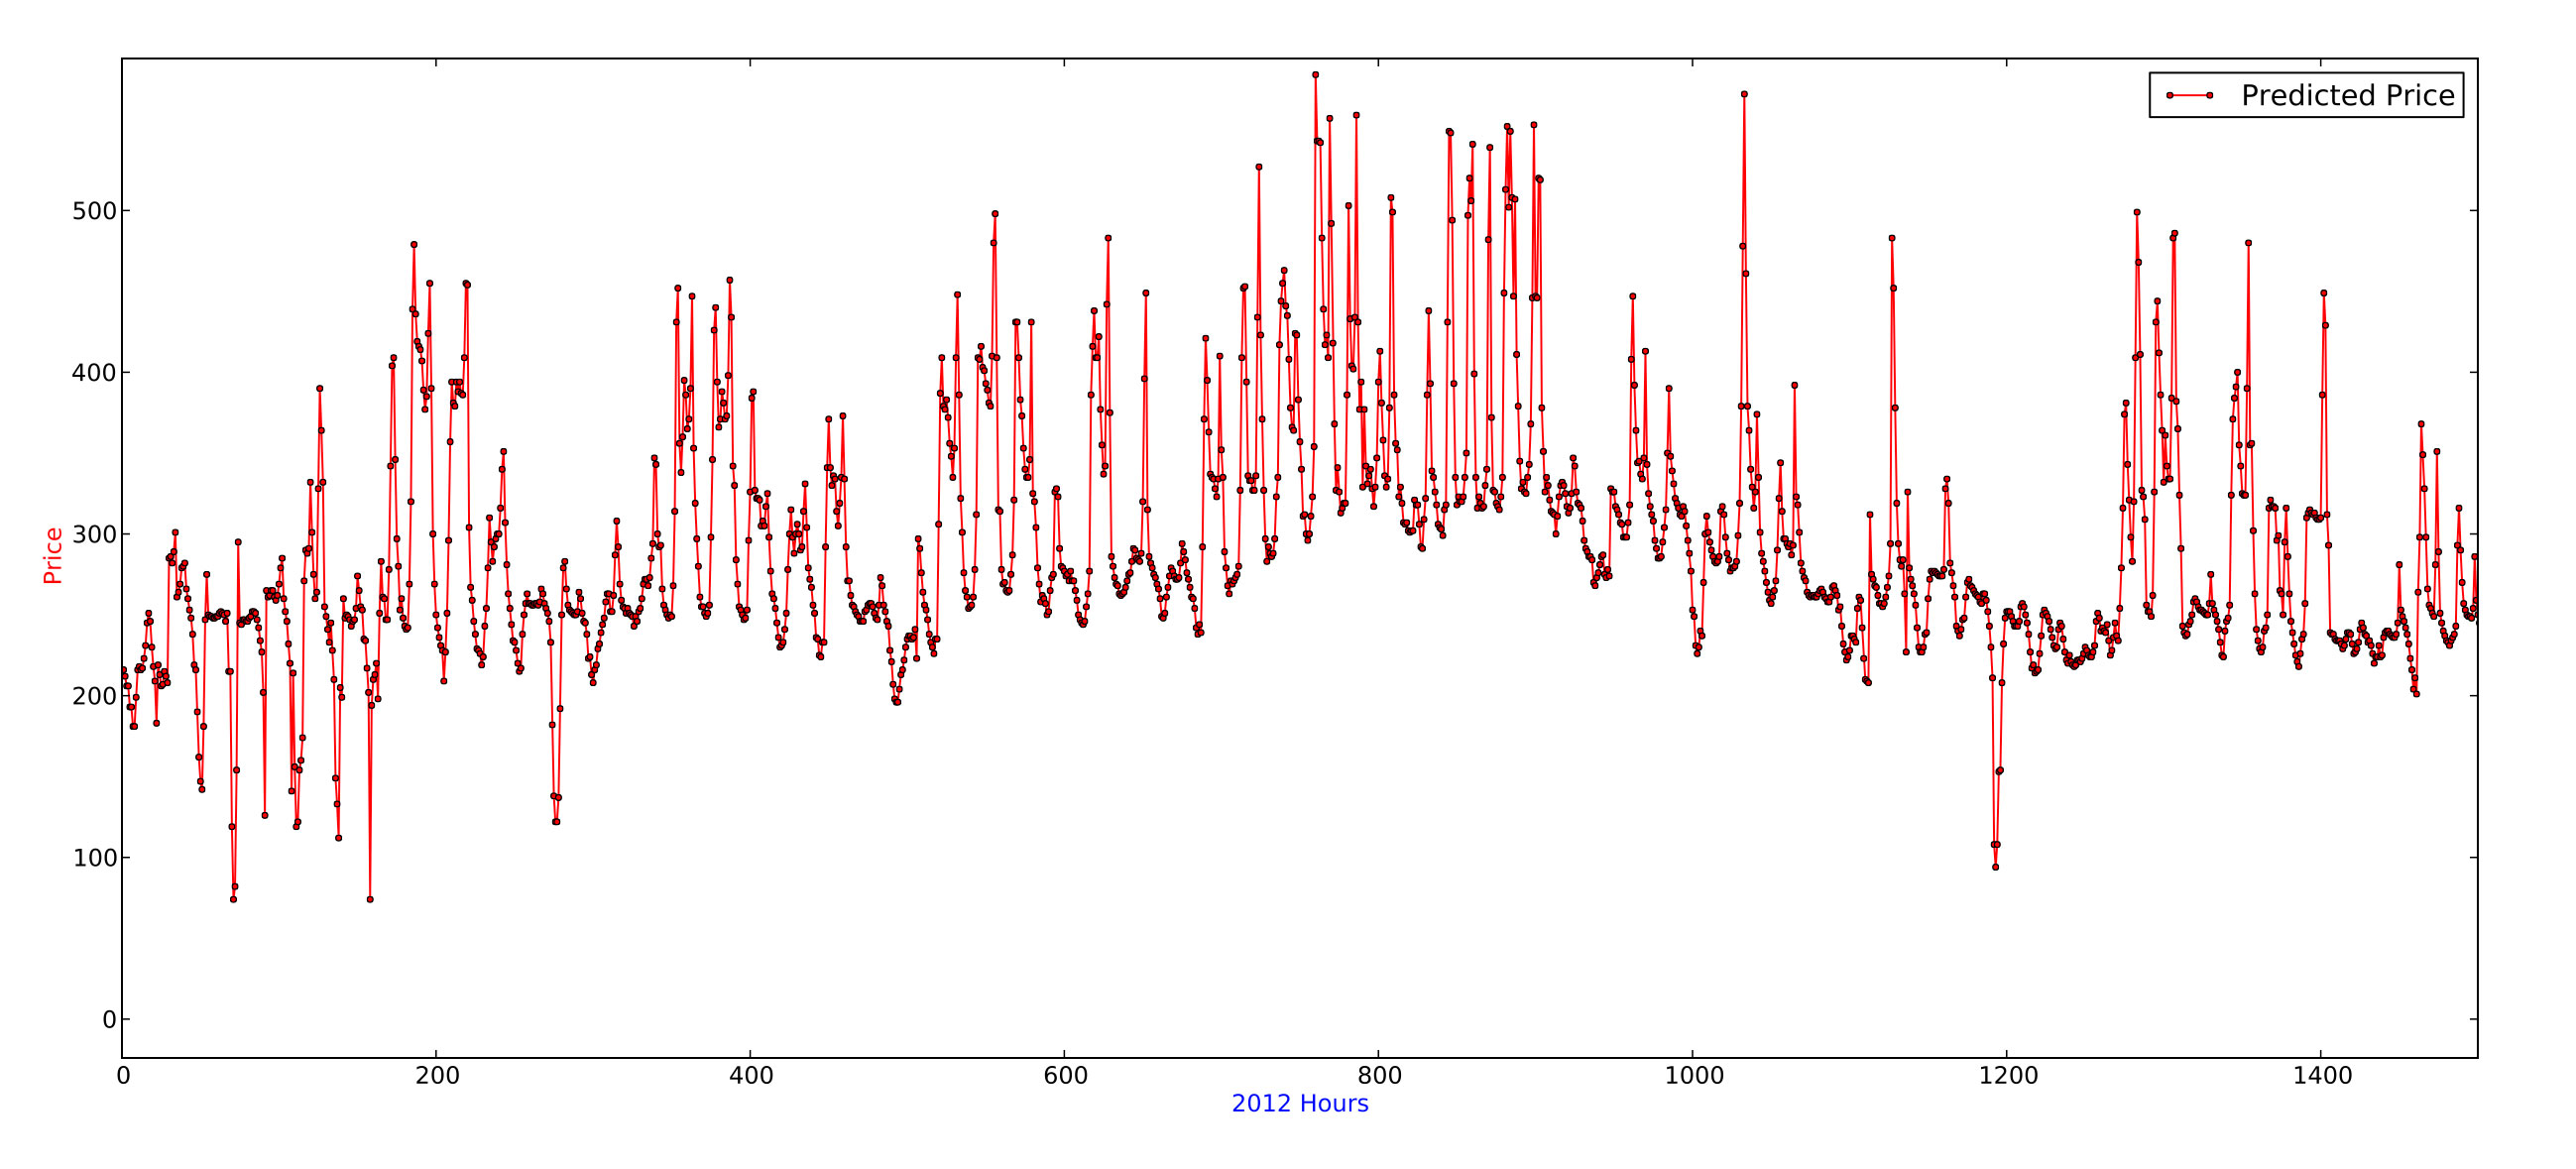
\includegraphics[width=\textwidth ]{billeder/energy_price_plots/plotGraph.jpg}
\caption{A plot graph of the price development over the first 1500 hours in 2012}
\label{fig:plotGraph}
\end{figure}

The volatility of the price is clearly shown in~\ref{fig:same_hour_distribution} where the price on similar hours fluctuates from 215 to 345. To address the volatile nature of the price we need to look at the trends of the known historical price. If we take a look at the price plot in figure~\ref{fig:plotGraph} it clearly shows how volatile the price actually is. Another thing we can derive from the graph is how the price moves. It doesn't just jump from top to bottom of the interval but it takes some steps to get there (in most cases). This tendency can be used alongside the last known price to give the neural network a direction to follow and an approximate price as a point of origin. For more details on this see section~\ref{sec:usingStatisticalInput}. As an example we can take a price of 250 and a rising tendency then we have pointers for the price development and we can in general discard every posibility of a price that is under 250 -- since the tendency was rising. We can also discard the highest of numbers since the price in general doesn't jump several hundred and therefore we will have an idea of where the price is heading even though it is very volatile.

In the same manner we can address the high-frequency spike prices that occurs in the time series. We have to identify a tendency in the historical data and use this to make the predictions follow the steep spikes in the dataset. The volatility is often easier to handle than the spike prices because the volatility most of the times only causes small jumps in the price and these are easier to predict.

\subsection{Demand}
Demand is directly connected to the energy prices (which comes as no suprise) since every market is driven by demand. Since demand is relative to the present time we are not able to use it directly as an input factor in the artificial neural network(ANN). We have a couple of choices here. We can take the demand from other instances like Nord Pool Spot; where they predict what the demand will be. We can compute the demand in artificial neural network and use the outputs as input for our price prediction ANN. At last we can try and substitute the demand input with the factors that plays a role in predicting the demand. The last two methods requires us to have an idea of what the input parameters for the prediction of demand is. As mentioned in related work we have seen a function that calculates the demand based on CDD(Cooling degree days), HDD(Heating degree days), ELD(Humidity), V$_w$ (Wind speed), M$_s$ (Sunshine), M$_r$ (Rainfall) \cite{19}. Based on this we will model the ANN to take the above mentioned factors as inputs.

\begin{figure}[H]
\centering
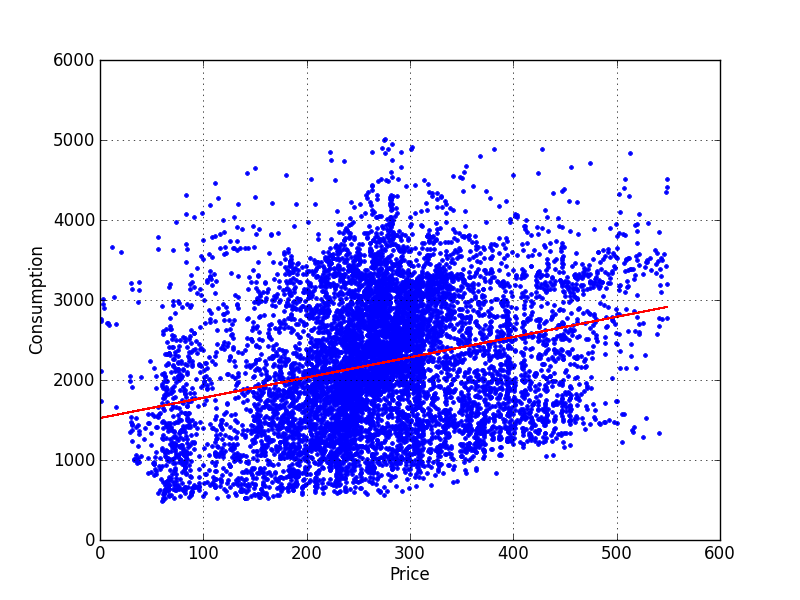
\includegraphics[width=0.8\textwidth ]{billeder/energy_price_plots/consump_price.png}
\caption{Demand and price plot.}
\label{fig:consump_price}
\end{figure}

In figure ~\ref{fig:consump_price} we see the connection between energy price and the demand. The model shows us that if the demand rises the price on the energy rises aswell. This is a common tendency in a market where there isn't endless supply. Since the price is heavily influenced by demand and demand is a relative factor the same calculations are also done by the powerplants because they need to know how much power to produce in a certain timeframe. We want to imitate this forecast and predict our own demand based on the aforementioned parameters. This is key to how accurate we will be able to predict the price. In other words: A good prediction of the demand will give us the right foundation for a good prediction of the price.

\begin{figure}[H]
\centering
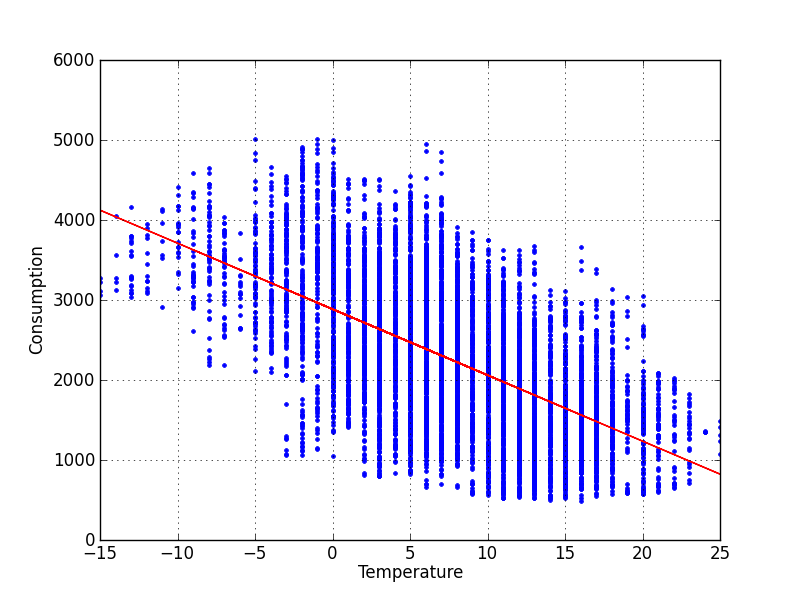
\includegraphics[width=0.8\textwidth ]{billeder/energy_price_plots/consump_temp.png}
\caption{Demand and temperature plot.}
\label{fig:consump_temp}
\end{figure}


In figure ~\ref{fig:consump_temp} we see the connection between demand and temperature. The temperature itself has an influence when it is very cold or very warm. This connection is expressed as CDD(Cooling degree days) and HDD(Heating degree days). In figure ~\ref{fig:consump_temp} we see that if temperature decreases the demand will go up. This is because the people of Denmark use a lot of energy on heating their homes and lighting them (HDD) in the winter time. In \cite{19} they also describe CDD which indicates the need for cooling. In Denmark it is limited how high the temperature goes and how often we actually need to cool our homes see table 

In our analysis of HDD and CDD we see that \todo{finish the CDD HDD}

\begin{figure}[H]
\centering
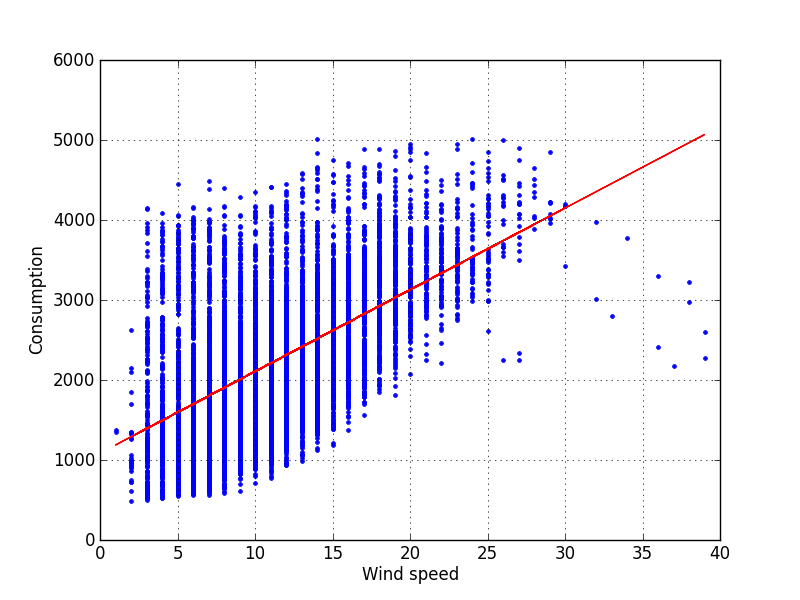
\includegraphics[width=0.8\textwidth ]{billeder/energy_price_plots/consump_wind.png}
\caption{Demand and wind speed plot.}
\label{fig:consump_wind}
\end{figure}

Wind speed plays a role in predicting electrical demand. The wind affects the electrical heating needed in homes across the country. The wind cools down the houses and thus need for heating arises \cite{19}. As seen in figure ~\ref{fig:consump_wind} and in table ~\ref{table:pearsonsPriceVariables} there is a pretty good correlation between wind speed and consumption. The graph clearly shows us that; when the wind speed increases (from 15 and up) the overall demand increases aswell. This indicates that high wind speeds will have th greatest influence on the demand.

TODO: Skriv om price development i forhold til graf udviklingen